
\section{Anforderungen}

Um die vorliegende Fragestellung zu beantworten, ist es notwendig mehrere Test zu verwenden, welche die Kompetenz des skalenbasierten Messens erheben. Zusätzlich müssen die Tests die Kompetenz des skalenbasierten Messens unter verschiedenen Kontexten ermitteln. Es wurden zwei existierende Test aus dem ExKoNawi Projekt verwendet. Der eine war aus dem Fachbereich Chemie, bei welchem eine Temperatur gemessen werden musste. Der zweite Test war aus dem Fachbereich Physik, bei dem eine Kraft bestimmt wurde. Zusätzlich wurde ein dritter Test neu entwickelt, bei welchem eine Temperaturmessung im Fach Physik durchgeführt wurde. Die Testerstellung wird  in \citet{Sichau2015} detailliert beschrieben. Der dritte Test wurde so entworfen, dass einmal der inhaltliche Kontext verändert werden kann (Kraftmessung versus Temperaturmessung), bei gleichem fachlichen Kontext und zum Anderen der fachliche Kontext verändert werden kann, ohne den inhaltlichen Kontext zu verändern. 


\section{Umsetzung}

Die Tests wurden zusammen mit einem Fragebogen an vier Klassen der Sek 1 A durchgeführt. In jeder Klasse wurden vier Gruppen gebildet, welche die Tests in unterschiedlicher Reihenfolge durchführten. Dafür gab es zwei Gründe. Zum einen war nur Material für 11 Tests verfügbar. Daher konnten die Tests nicht in voller Klassenstärke durchgeführt werden. Dies führte zur Bildung von zwei Gruppen, wobei eine zuerst den Fragebogen ausfüllte und die andere Gruppe den Fragebogen am Ende ausfüllte. Zusätzlich wurde noch der zweite und dritte Test in jeder Gruppe vertauscht, um zu untersuchen, ob Müdigkeit oder die Wiederholungen Einfluss auf die Test-Ergebnisse haben. Die Tabelle \ref{tab:Gruppenaufteilung} gibt eine Übersicht über die Gruppeneinteilung der Schülerinnen und Schüler innerhalb einer Klasse.
\begin{table}[htbp]
  \centering
  \begin{tabular}{@{}p{3.1cm}p{3.1cm}p{3.1cm}p{3.1cm}@{}}
  \toprule
   Gruppe FABC & Gruppe FACB & Gruppe ABCF & Gruppe ACBF \\ 
  \midrule
   Fragebogen & Fragebogen & Temperatur \newline  Physik 305 & Temperatur \newline  Physik 305 \\[0.2cm]
   Temperatur \newline  Physik 305 & Temperatur \newline  Physik 305 & Kraft \newline  Physik & Temperatur Chemie \\ [0.2cm]
   Kraft  \newline Physik 301 & Temperatur \newline  Chemie 201 & Temperatur \newline  Chemie 201 & Kraft \newline  Physik 301 \\ [0.2cm]
   Temperatur \newline  Chemie 201 & Kraft \newline  Physik 301 & Fragebogen& Fragebogen\\ 
   
  \bottomrule
  \end{tabular} 
  \caption{Aufteilung der Gruppen innerhalb einer Klasse}
  \label{tab:Gruppenaufteilung}
\end{table}

Die Namen der Gruppen aus Tabelle \ref{tab:Gruppenaufteilung} wurden auch für die Kodierung der Tests verwendet, sodass jeder Test einer Gruppe zuordenbar ist.

Die vier Klassen waren alle von derselben Schulstufe (7. Schuljahr), jedoch stammten sie aus verschiedenen Gemeinden. Die Klassen in Glattbrugg hatten beide dieselbe Lehrperson, die anderen Klassen hatten unterschiedliche Lehrpersonen. Ein Überblick über die wichtigsten Daten zu den einzelnen Klassen lässt sich der Tabelle \ref{tab:Klassen} entnehmen. 


\begin{table}[htbp]
  \centering
  \begin{tabular}{@{}lp{2.3cm}p{3cm}p{3cm}p{3cm}p{3cm}@{}}
  \toprule
   & Klasse 1 & Klasse 2 & Klasse 3 & Klasse 4 \\ 
  \midrule
   Ort & Glattbrugg & Glattbrugg & Stadt Zürich & Stadt Schaffhausen \\ [0.2cm]
   Anzahl SuS & 15 & 13 (+1 nur einen Test) & 22 & 22 \\ [0.2cm]
   Datum  & 6.11.14 & 6.11.14 & 12.11.14 & 11.12.14\\ [0.3cm]
   Uhrzeit & 8:20-10:00 & 10:20-12:00& 10:20-12:05 & 13:15-14:45 \\ [0.3cm]
   Versuchsleiter & Pitt Hild und David Sichau   & Pitt Hild und David Sichau  & Pitt Hild und David Sichau  & Martina Minges und David Sichau \\
  \bottomrule
  \end{tabular} 
  \caption{Wichtigste Informationen zu den einzelnen Klassen}
  \label{tab:Klassen}
\end{table}

Alle Klassen wurden für die Durchführung in zwei Gruppen aufgeteilt. Zum einen konnten so die Schülerinnen und Schüler mit mehr Abstand positioniert werden, um die Ablenkung zu reduzieren. Andererseits konnten so die Schülerinnen und Schüler, welcher der Videoaufnahme nicht zugestimmt hatten, in ein Zimmer gesetzt werden, indem keine Videoaufnahme stattfand hat. Die Erlaubnis zur Videoaufnahme wurde bereits vor der Durchführung von den Klassenpersonen organisiert und eingesammelt.



\section{Untersuchung}

\subsection{Vorbereitung}
Für die Durchführung in den einzelnen Klassen wurden alle Tests in Boxen vorbereitet, sodass zwischen den Tests nur die Boxen ausgetauscht werden mussten. In jeder Box waren alle Materialien, welche für die Durchführung des Versuches notwendig waren, vorbereitet, sodass die Schülerinnen und Schüler alle benötigten Materialien in dieser Box finden konnten.  

\begin{figure}[htb]
\centering
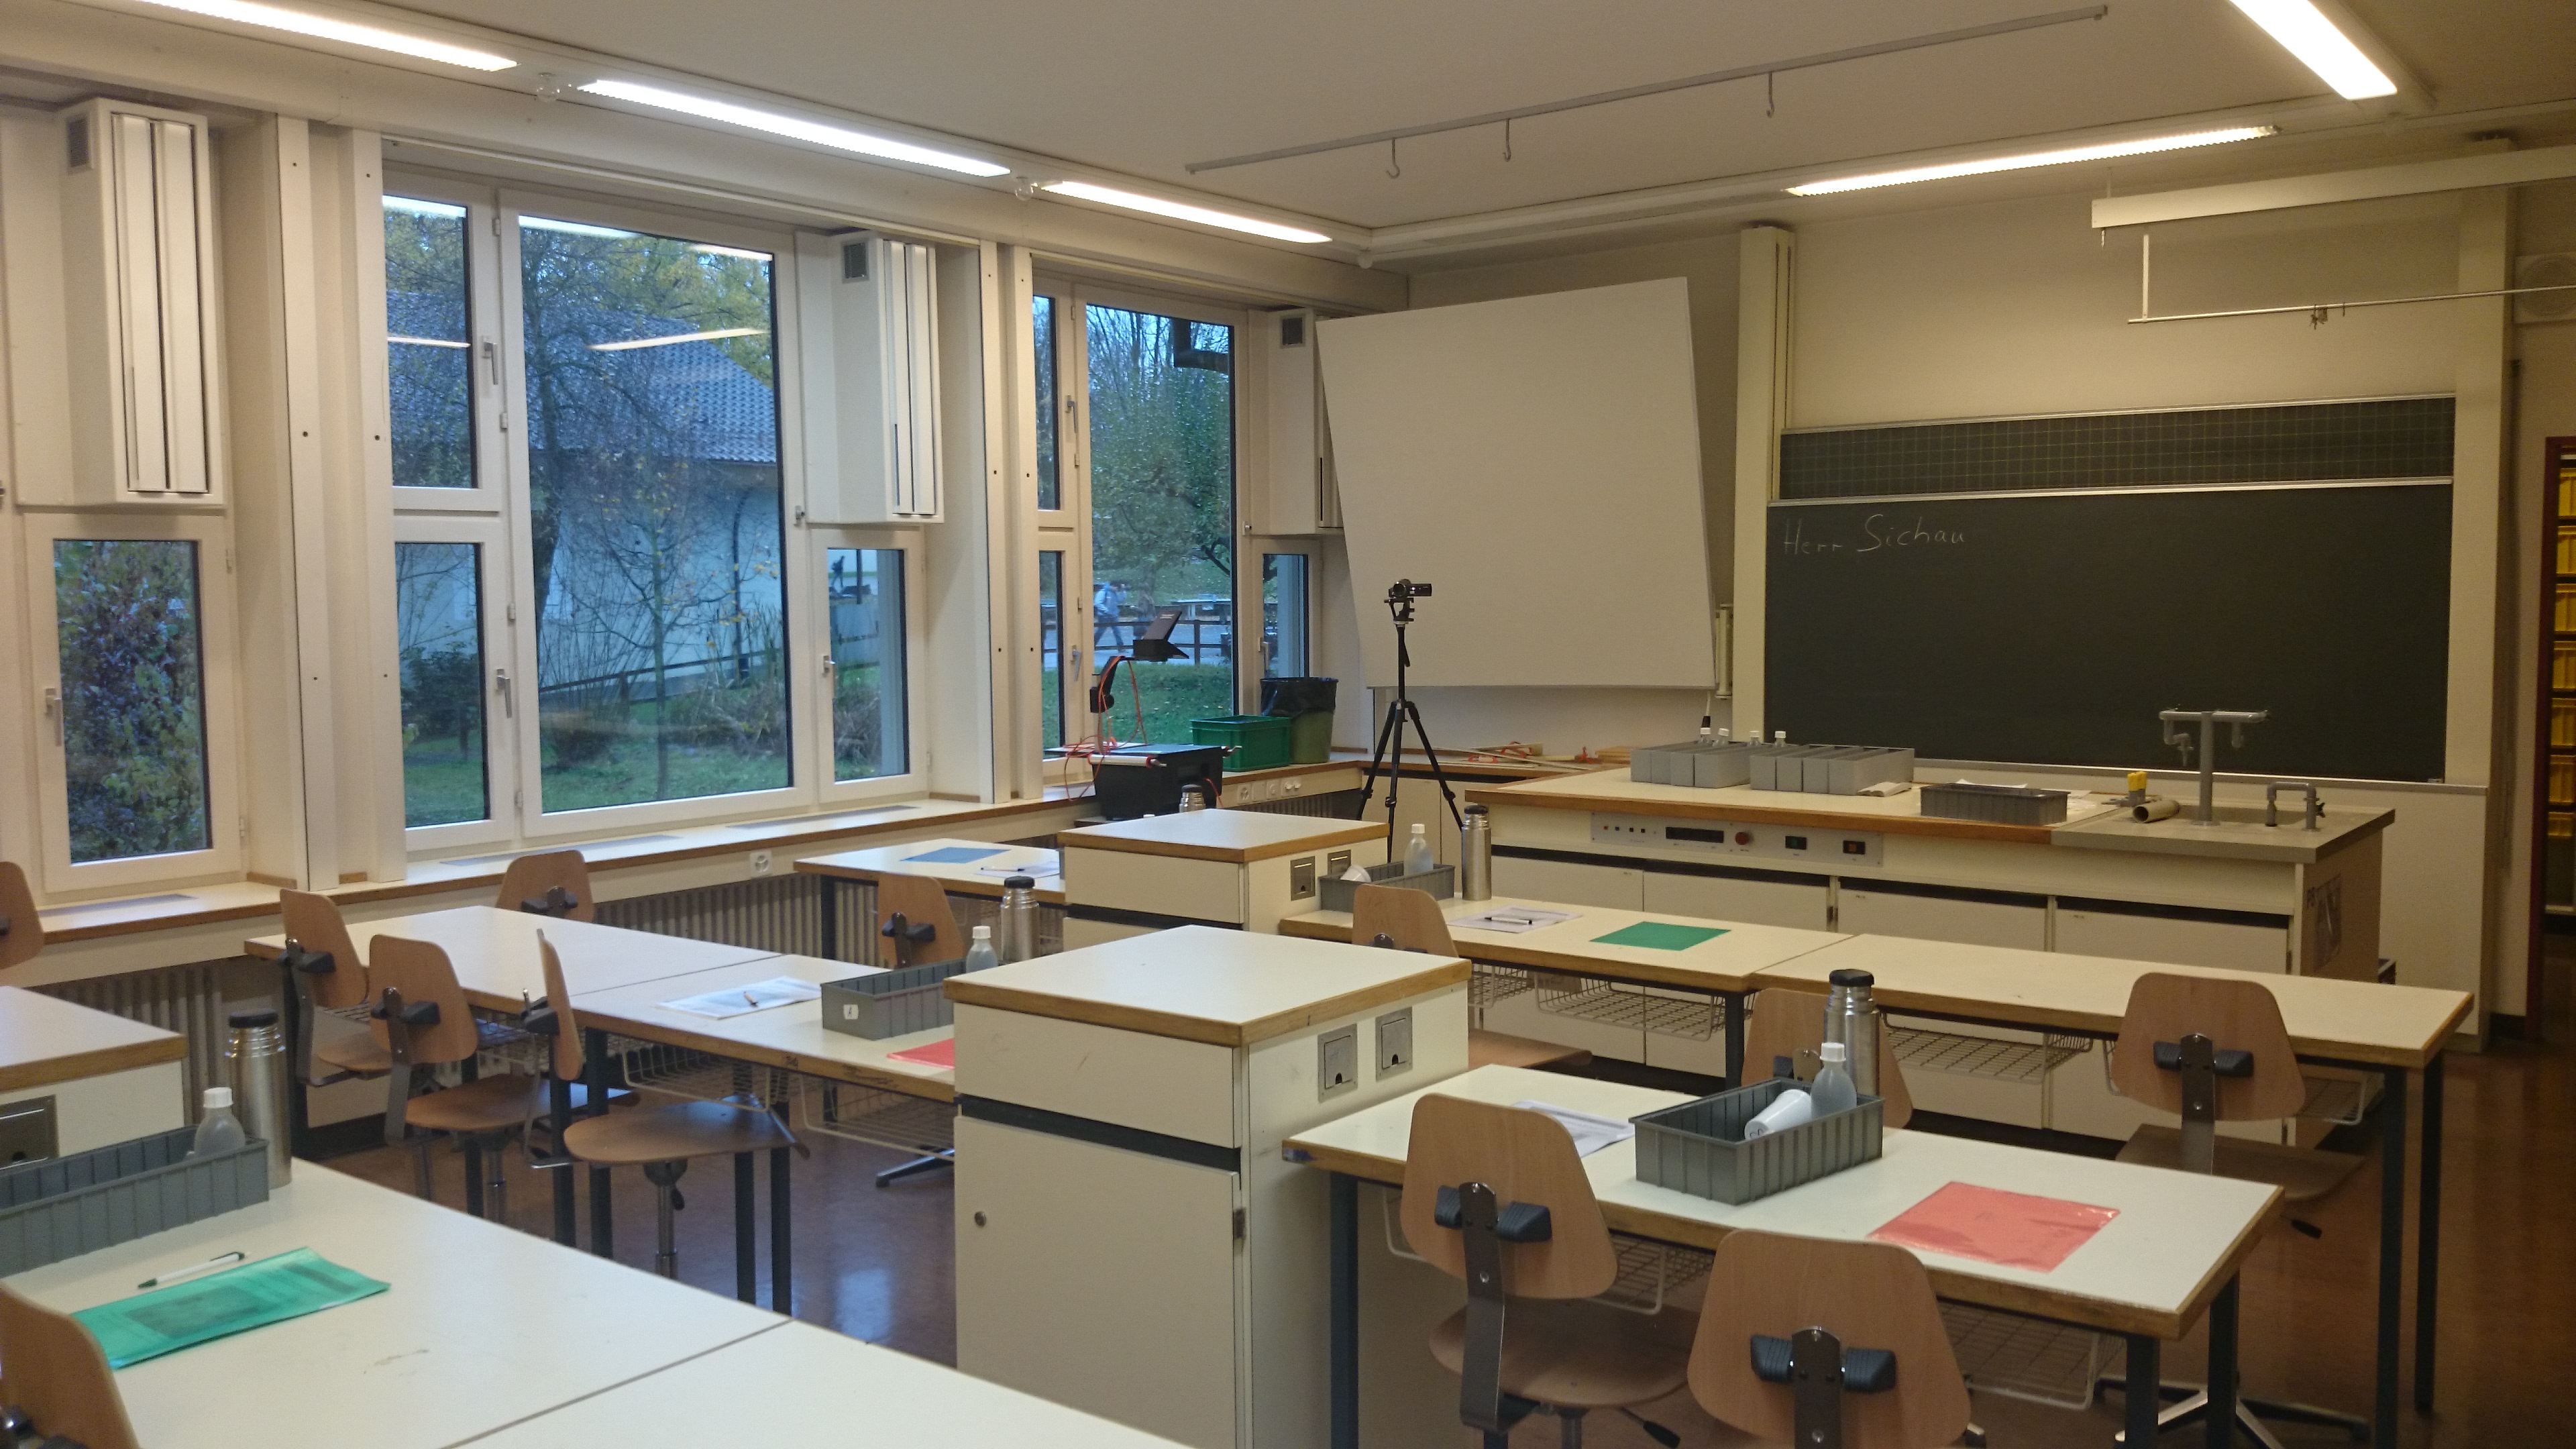
\includegraphics[width=0.98\linewidth]{graphics/Durchfuerhung}
\caption[Vorbereitetes Klassenzimmer.]{Klassenzimmer für die Durchführung des ersten Durchganges vorbereitet.}
\label{fig:Durchfuerhung}
\end{figure}

Zusätzlich wurden die Auswertungsbögen in der richtigen Reihenfolge und bereits mit einer Kodierung versehen in einem Schnellhefter bereitgestellt. Ein für die Durchführung vorbereiteter Klassenraum ist im Bild \ref{fig:Durchfuerhung} ersichtlich.

Im Bild \ref{fig:Durchfuerhung} sieht man auch gut, wie die Kamera für die Videoauswertung aufgestellt wurde. Die Videoaufnahme wurde vor Eintreten der Schülerinnen und Schüler gestartet, um die Ablenkung durch die Kamera möglichst gering zu halten.

\subsection{Durchführung}
Nachdem die Schülerinnen und Schüler in die beiden Räume aufgeteilt wurden, wurden sie von den Versuchsleitern jeweils begrüsst. Die Begrüssung war stichwortartig vorbereitet, damit alle Klassen die gleichen Informationen erhielten und durch die Begrüssung die Testergebnisse nicht beeinflusst werden konnten. Dabei wurde darauf hingewiesen, dass die Experimente keine Leistungskontrolle darstellt und alle Ergebnisse anonymisiert sind. Es wurde auch ein grober Überblick über den Ablauf gegeben. Im Raum, in dem eine Videoaufnahme gemacht wurde, wurden die Schülerinnen und Schüler darüber informiert. 

Nach der Begrüssung wurden die Schülerinnen und Schüler aufgefordert mit den Tests anzufangen. Während der Zeit, in welcher die Tests durchgeführt wurden, gaben die Versuchsleiter jeweils kurze Zeit Informationen und forderten die Schülerinnen und Schüler auf ihre Ergebnisse zu verschriftlichen.

Nach dem ersten Test (nach 20 Minuten) wurde eine Pause von fünf Minuten durchgeführt. In dieser wurden die Boxen ausgetauscht, sodass alle Schülerinnen und Schüler den nächsten hands-on Experimentiertest vor sich hatten. Die Schülerinnen und Schüler wurden aufgefordert sich innerhalb des Klassenraumes zu bewegen. Nach dem zweiten Test wurde eine grosse Pause durchgeführt, in welcher die Schülerinnen und Schüler das Schulzimmer verlassen konnten. Nach dem dritten Test wurde wieder eine kurze fünfminütige Pause durchgeführt. Während der Tests wurden den Schülerinnen und Schülern nur Fragen zu Unklarheiten beantwortet, inhaltliche Fragen oder Fragen zum korrekten Vorgehen wurden zurückgewiesen. 

\subsection{Nachbereitung}

Nachdem die Tests durchgeführt wurden, wurden die Auswertungsbögen eingesammelt und von David Sichau erstkodiert. Es wurde eine Zweitkodierung vor 15 \% der Auswertungsbögen von Pitt Hild durchgeführt. Die 11 Auswertungsbögen zur Zweitkodierung wurden zufällig (random generator) ausgewählt, um sicherzugehen, dass ein Bias ausgeschlossen werden kann. Insgesamt wurden 72 Auswertungsbögen vollständig ausgefüllt. 

Die Videoaufnahmen wurden geschnitten, sodass nur noch die einzelnen Tests sichtbar sind. Dies wurde gemacht, um zu vermeiden, dass Aktionen der Schülerinnen und Schüler in der Pause einen Einfluss auf die Bewertung in der Testsituation hatten. Insgesamt ist Material zu 8 Schülerinnen und Schüler verwertbar, da die andern zu weit entfernt sind und daher ihre Aktionen nicht beobachtbar waren.

